\documentclass{homework}
\author{Joseph Siu}
\class{MAT157: Analysis I}
\date{\today}
\title{Homework 2}


\theoremstyle{remark}
\newtheorem*{claim}{Claim}
\newtheorem*{definition}{Definition}

% Symbols
\newcommand*{\eg}{\leavevmode\unskip , e. g., \ignorespaces}
\newcommand*{\ie}{\leavevmode\unskip, i. e., \ignorespaces}
\newcommand{\nil}{\varnothing}
\AtBeginDocument{\def\O{\cal{O}}} % Big Oh
\AtBeginDocument{\def\C{\bb{C}}} % Complex
\newcommand{\R}{\bb{R}} % Reals
\newcommand{\Q}{\bb{Q}} % Rationals
\newcommand{\Z}{\bb{Z}} % Integers
\newcommand{\N}{\bb{N}} % Naturals
\renewcommand{\P}{\bb{P}} % Primes
\newcommand{\F}{\bb{F}} % Field
\newcommand{\GF}[1][2]{\bb{F}_{#1}} % Galois Field
\newcommand{\modulo}[1][n]{\Z/#1\Z} % Modulo class n
\newcommand{\ra}{\rightarrow}
\newcommand{\Ra}{\Rightarrow}
\newcommand{\?}{\stackrel{?}{=}}
\newcommand{\is}{\equiv}
\newcommand{\al}{\alpha}
\newcommand{\ep}{\varepsilon}
\renewcommand{\phi}{\varphi}
\newcommand{\p}{\partial}
\newcommand{\injective}{\hookrightarrow}
\newcommand{\surjective}{\twoheadrightarrow}
\newcommand{\bijective}{\hookrightarrow\mathrel{\mspace{-15mu}}\rightarrow}
\newcommand{\derivative}[2][x]{\frac{\D #2}{\D #1}}
\newcommand{\ceil}[1]{\left\lceil#1\right\rceil}
\newcommand{\floor}[1]{\left\lfloor#1\right\rfloor}
\newcommand{\near}[1]{\left\lfloor#1\right\rceil}
\newcommand{\arr}[1]{\left\langle#1\right\rangle}
\newcommand{\paren}[1]{\left(#1\right)}
\newcommand{\brk}[1]{\left[#1\right]}
\newcommand{\abs}[1]{\left|#1\right|}
\newcommand{\curl}[1]{\left\{#1\right\}}

\begin{document} \maketitle

\section*{Exercise 1}
Determine if each of the following statement is true or false. Prove your claim. 

\question Let $A,B,C$ be any three sets. If $A=B,$ then $A\times C=B\times C.$ 
\begin{claim}
    Let $A,B,C$ be any three sets. If $A=B,$ then $A\times C=B\times C.$ 
\end{claim}
\begin{proof}
    We want to show $A\times C\subseteq B\times C$ and $A\times C \supseteq B\times C$.
    
    Firstly, by the definition, $A=B$ implies $A\subseteq B$ and $B\subseteq A$. Pick any $(a,c)\in A\times C$ which $a\in A$ and $c\in C$, then we know that $A\subseteq B\implies a\in B$, this follows $(a,c)\in B\times C$, showing $A\times C\subseteq B\times C$. 

    Secondly, letting $(b,c)\in B\times C$ which $b\in B$ and $c\in C$, then we know that $B\subseteq A\implies b\in A$, this follows $(b,c)\in A\times C$, showing $B\times C\subseteq A\times C$. 
    
    By definition, when $A\times C\subseteq B\times C$ and $B\times C\subseteq A\times C,$ we can say $A\times C = B \times C$. 
\end{proof}

%%this is actually false
\question Let $A,B,C$ be any three sets. If $A\times C=B\times C,$ then $A=B$.
\begin{claim}
    Let $A,B,C$ be any three sets. If $A\times C=B\times C,$ then $A=B$.
\end{claim}
\begin{proof}
    When $A\times C = B \times C,$ by definition, $A\times C\subseteq B\times C$ and $B\times C\subseteq A\times C$. We want to show that $A\subseteq B$ and $A\supseteq B$. 

    First, pick any $(a,c)\in A\times C$, this means $a\in A$ and $c\in C$. By the definition of subset, $A\times C\subseteq B\times C \implies (a,c)\in B\times C$, this gives $a\in B$ and $c\in C$, showing $A\subseteq B$. 

    Second, pick any $(b,c)\in B\times C$, this means $b\in B$ and $c\in C$. By the definition of a subset, $B\times C\subseteq A\times C \implies (b,c)\in A\times C$, this gives $b\in A$ and $c\in C$, showing $B\subseteq A$. 

    Therefore, since $A\subseteq B$ and $B\subseteq A$, by definition, $A=B$, as required.
\end{proof}

\question Let $A,B,C$ be any three sets. If $(A\times B)\cup(B\times A)=C\times C,$ then $A\cap B=C.$
\begin{claim}
   Let $A,B,C$ be any three sets. If $(A\times B)\cup(B\times A)=C\times C,$ then $A\cap B=C.$
\end{claim}
\begin{proof}
    We prove this statement by showing the contrapositive is true. i.e., $A\cap B\neq C \implies (A\times B)\cup(B\times A)\neq C\times C$. When $A\cap B\neq C$, by the definition, $A\cap B\not\subseteq C\lor C\not\subseteq A\cap B$. 

    \underline{Case $A\cap B\not\subseteq C$}: This implies $\exists x\in A\cap B, x\notin C$, that is, $x\in A\cap B\implies x\in A \land x\in B\implies (x,x)\in A\times B \land (x,x)\in B\times A\implies (x,x)\in (A\times B)\cup (B\times A)$, but $x\notin C\implies (x,x)\notin C\times C$. This shows $(A\times B)\cup (B\times A)\not\subseteq C\times C$, thus by the definition, $(A\times B)\cup(B\times A)\neq C\times C$ as required. 

    \underline{Case $C\not\subseteq A\cap B$}: This implies $\exists x\in C, x\notin A\cap B$, that is, $x\in C\implies (x,x)\in C\times C$, but $x\notin A\cap B\implies (x,x)\notin A\times B\land (x,x)\notin B\times A\implies (x,x)\notin (A\times B)\cup(B\times A)$. This shows $C\times C\not\subseteq (A\times B)\cup(B\times A)$, thus by definition, $(A\times B)\cup(B\times A)\neq C\times C$ as required.

    We have shown that $A\cap B\neq C \implies (A\times B)\cup(B\times A)\neq C\times C$ for all cases, therefore, the contrapositive is true, implying the statement is also true.
\end{proof}


% \begin{proof}
% First assume for the sake of contradiction, the statement is true, i.e., By definition, $(A\times B)\cup(B\times A)=C\times C$ implies $C\times C\subseteq(A\times B)\cup(B\times A)$ i.e., $(\forall c\in C)(\exists a\in A)(\exists b \in B)((c,c)=(a,b)\lor(c,c)=(b,a))$. Fix an element $x\in C$ s.t. $x\notin A \land x\notin B$. Since $(\exists a\in A)(\exists b \in B)((x,x)=(a,b)\lor(x,x)=(b,a))$, this means $(x=a\land x=b)\lor(x=b\land x=a)$, which follows $(x\in A\land x\in B)\lor(x\in B\land x\in A)$, but as we previously fixed $x$ to be $x\notin A$ and $x \notin B$, $(x\in A\land x\in B)$ and $(x\in B\land x\in A)$ are both false and so is $(x\in A\land x\in B)\lor(x\in B\land x\in A)$, i.e., $(x\in A\land x\in B)\lor(x\in B\land x\in A)$ being false contradicting it is true, therefore, the statement is false, the claim holds. 
% \end{proof}



\question Let $A,B,C$ be any three sets. If $A\cap B=C,$ then $(A\times B)\cup(B\times A)=C\times C.$ 
\begin{claim}
The statement "Let $A,B,C$ be any three sets. If $A\cap B=C,$ then $(A\times B)\cup(B\times A)=C\times C.$ " is false. 
\end{claim}
\begin{proof}
    We prove the question is false by showing a counterexample. Let $A=\{1,2\}, B=\{2,3\}, C=\{2\}.$ i.e. $A\cap B=\{1,2\}\cap\{2,3\}=\{2\}.$ Showing $A\cap B=\{2\}\subseteq \{2\}=C$ and $C=\{2\}\subseteq \{2\}=A\cap B,$ by the definition $A\cap B = C$. But then,  
    \begin{align*}
    (A\times B)\cup(B\times A)&=\{(1,2),(1,3),(2,2),(2,3)\}\cup\{(2,1),(2,2),(3,1),(3,2)\}\\&=\{(1,2),(1,3),(2,1),(2,2),(2,3),(3,1),(3,2)\},
\end{align*}
and $C\times C=\{(2,2)\},$ because $$(A\times B)\cup(B\times A)=\{(1,2),(1,3),(2,1),(2,2),(2,3),(3,1),(3,2)\}\not\subset\{(2,2)\},$$ therefore $(A\times B)\cup(B\times A)\neq C\times C$ by the definition. 
\end{proof}




\newpage
\section*{Exercise 2}
\question Given the set $X=\{1,2,3,4,\ldots,2024\}$ and its power set $\mathcal{P}(X),$ define the set $$A=\{(x,y)\in\mathcal{P}(X)\times\mathcal{P}(X)\mid x\subsetneq y\}.$$ How many elements are there in $A$? (You can provide your final answer as a summation.) 

\begin{claim}
    Given the set $X=\{1,2,3,4,\ldots,2024\}$ and its power set $\mathcal{P}(X)$, define the set $$A=\{(x,y)\in\mathcal{P}(X)\times\mathcal{P}(X)\mid x\subsetneq y\}.$$ The number of elements of $A$ is $$\sum_{i=0}^{2024}\frac{(2^i-1)\cdot2024!}{i!(2024-i)!}.$$
\end{claim}
\begin{proof}
First, we know that for a set containing $n$ elements, it has $2^n$ subsets, including itself. i.e., the number of elements in the power set of the set is also $2^n$ and the number of proper subset is $2^n-1.$ Given the set $X=\{1,2,3,4,\ldots,2024\},$ we know that its power set $\mathcal{P}(X)$ contains $2^{2024}$ elements. In order to find the number of elements in $A,$ we can separate the cases of $y$:

We notice that $(x,y)\in\mathcal{P}(X)\times\mathcal{P}(X)\implies y\in\mathcal{P}(X)$. Let $i$ be the number of elements of $y$, since the number of elements of $X$ is 2024, so $i\in\mathbb{Z}\cap[0,2024]$. By the binomial theorem, we use $_{2024}C_{i} \iff \frac{2024!}{i!(2024-i)!}$ to determine the number of combinations we can pick $i$ elements from 2024 elements.  $\sum_{i=0}^{2024}\frac{2024!}{i!(2024-i)!}$ gives the total number of subsets of $X,$ which using calculator to verify we can find out that it is same as $2^{2024}.$ 

Now, we want to figure out how many possibilities for $x$ there are for $y$ with different number of elements. Since we defined $x$ to be the proper subset of $y$ which $x\subsetneq y,$ and $(x,y)\in\mathcal{P}(X)\times\mathcal{P}(X)\implies x\in\mathcal{P}(X)$. So, we want to figure out how many proper subsets $y$ has, as previously determined, there are $2^i-1$ proper subsets for $y$ containing $i$ elements. 

So, with the two formulas $\sum_{i=0}^{2024}\frac{2024!}{i!(2024-i)!}$ and $2^i-1$ we can figure out how many elements the set $A$ have, i.e., when we know $y$ has $i$ elements, there are $2^i-1$ possibilities for $x$ which means in this case there are $2^i-1$ elements in $A$, after that, we notice that there are $\frac{2024!}{i!(2024-i)!}$ different possibilities for $y$ which contains $i$ elements, multiplying $2^i-1$ and $\frac{2024!}{i!(2024-i)!}$ , $(2^i-1)\cdot\frac{2024!}{i!(2024-i)!}$, gives the total number of elements in $A$ which the $y$ of all elements all contain $i$ elements respectively. Because the number of elements of the elements of $A$ can vary from $0$ to $2024,$ we sum up the $i$ from 0 to 2024 to get the total number of elements of $A$ with all possibilities of $x$ and $y$, $$\sum_{i=0}^{2024}(2^i-1)\cdot\frac{2024!}{i!(2024-i)!} = \sum_{i=0}^{2024}\frac{(2^i-1)\cdot2024!}{i!(2024-i)!}.$$ Therefore, we have proven our claim. 
\end{proof}

\newpage
\section*{Exercise 3}
Let $f:A\rightarrow B$ be a function. For any set $C\subseteq A$ and $D\subseteq B$, Determine if each of the following statement is true or false. Prove our claim. 
\question For any $C_1,C_2\subseteq A, f(C_1\cap C_2)=f(C_1)\cap f(C_2)$.
\begin{claim}
    The statement "For any $C_1,C_2\subseteq A, f(C_1\cap C_2)=f(C_1)\cap f(C_2)$" is false. 
\end{claim}
\begin{proof}
    We show this statement is false by showing a counterexample. 

    Let $f: \mathbb{R}\rightarrow \mathbb{R}, f(x)=x^2$. Pick $C_1=[-1,0]\in\mathbb{R}$ and $C_2=[0,1]\in\mathbb{R}$. i.e., $f(C_1\cap C_2)=f([-1,0]\cap[0,1])=f(\{0\})=\{0\},$ and $f(C_1)\cap f(C_2)=f([-1,0])\cap f([0,1])=[0,1]\cap[0,1]=[0,1],$ we can clearly see that $[0,1]\not\subseteq\{0\}$. Therefore, by definition this is a valid counterexample showing the statement is false. 
\end{proof}



% \begin{proof}
%    \textbf{[redundant]} We show the statement is false by showing the negation of the statement is true. The negation of the statement is "There exist $C_1,C_2\subseteq A, f(C_1\cap C_2)\neq f(C_1)\cap f(C_2)$".  To show the negation statement is true, by negating the definition of the equality of sets, this is equivalent to show that $f(C_1\cap C_2)\not\subseteq f(C_1)\cap f(C_2) \lor f(C_1)\cap f(C_2)\not\subseteq f(C_1\cap C_2)$ is true for some $C_1, C_2 \subseteq A$. 
    
%     \underline{$f(C_1)\cap f(C_2)\not\subseteq f(C_1\cap C_2)$}: Choose an element $b\in B \text{ s.t. } b\in f(C_1)\cap f(C_2)$ and fixing $c_1,c_2\in A$, $(\forall c_4,c_5\in A)(f(c_4)=f(c_5)=b\implies c_4\in\{c_1, c_2\}\land c_5\in\{c_1, c_2\})$. This follows $b\in f(C_1)\land b\in f(C_2)$. We pick $C_1, C_2\subseteq A$ s.t. $c_1\in C_1 \land c_2\in C_2 \land c_1\notin C_2 \land c_2\notin C_1$. i.e., $c_1\notin C_1\cap C_2$ since $c_1\notin C_2$ and $c_2\notin C_1\cap C_2$ since $c_2\notin C_1$. This implies $b\notin f(C_1)\cap f(C_2)$. An element in $f(C_1)\cap f(C_2)$ is not in $f(C_1\cap C_2)$, showing $f(C_1)\cap f(C_2)\not\subseteq f(C_1\cap C_2)$, as required. 

%     Thus, as $f(C_1)\cap f(C_2)\not\subseteq f(C_1\cap C_2)$ is true, $f(C_1\cap C_2)\not\subseteq f(C_1)\cap f(C_2) \lor f(C_1)\cap f(C_2)\not\subseteq f(C_1\cap C_2)$ also holds true, proving the negation of the statement is true which implies the statement is false.

%     Therefore, the claim holds true as required. 
     
% \end{proof}



\question For any $C_1, C_2 \subseteq A, f(C_1\setminus C_2)=f(C_1)\setminus f(C_2)$. 
\begin{claim}
    The statement "$C_1, C_2 \subseteq A, f(C_1\setminus C_2)=f(C_1)\setminus f(C_2)$" is false.
\end{claim}
\begin{proof}
    We show this statement is false also by counterexample.  
    
    Let $f: \mathbb{R}\rightarrow \mathbb{R}, f(x)=x^2$. Pick $C_1=[-1,0]\in\mathbb{R}$ and $C_2=[0,1]\in\mathbb{R}$. i.e., $f(C_1\setminus C_2)=f([-1,0]\setminus[0,1])=f([-1,0))=(0,1]$ and $f(C_1)\setminus f(C_2)=f([-1,0])\setminus f([0,1])=[0,1]\setminus[0,1]=\emptyset$. We can see that $(0,1]\not\subseteq\emptyset$, therefore, by definition this is a valid counterexample showing the statement is false. 
\end{proof}
\question For any $D_1, D_2 \subseteq B, f^{-1}(D_1\cup D_2)=f^{-1}(D_1)\cup f^{-1}(D_2).$ 
\begin{claim}
    For any $D_1, D_2 \subseteq B, f^{-1}(D_1\cup D_2)=f^{-1}(D_1)\cup f^{-1}(D_2).$ 
\end{claim}
\begin{proof}
    To show $D_1, D_2 \subseteq B, f^{-1}(D_1\cup D_2)=f^{-1}(D_1)\cup f^{-1}(D_2)$, by definition, this is equivalent to show $f^{-1}(D_1\cup D_2)\subseteq f^{-1}(D_1)\cup f^{-1}(D_2)$  and $f^{-1}(D_1\cup D_2)\supseteq f^{-1}(D_1)\cup f^{-1}(D_2)$. 

    \underline{$f^{-1}(D_1\cup D_2)\subseteq f^{-1}(D_1)\cup f^{-1}(D_2)$}:  Pick an arbitrary element $c\in f^{-1}(D_1\cup D_2),$ by the definition of the image of a function, $f(c)\in D_1\cup D_2,$ i.e., $f(c)\in D_1\cup D_2 \iff f(c)\in D_1 \lor f(c)\in D_2$, by the definition of the pre-image of a function, $c\in f^{-1}(D_1)\lor c\in f^{-1}(D_2)\iff c\in f^{-1}(D_1)\cup f^{-1}(D_2)$. Showing that $f^{-1}(D_1\cup D_2)\subseteq f^{-1}(D_1)\cup f^{-1}(D_2)$ as required. 

    \underline{$f^{-1}(D_1\cup D_2)\supseteq f^{-1}(D_1)\cup f^{-1}(D_2)$}: Pick an arbitrary element $c\in f^{-1}(D_1)\cup f^{-1}(D_2)$, this is equivalent to $c\in f^{-1}(D_1)\lor c\in f^{-1}(D_2)$, by the definition, $f(c)\in D_1 \lor f(c)\in D_2\iff f(c)\in D_1\cup D_2$, by the definition, $c\in f^{-1}(D_1\cup D_2)$. Showing that $f^{-1}(D_1\cup D_2)\supseteq f^{-1}(D_1)\cup f^{-1}(D_2)$ as required. 

    Therefore, by the definition of the equality of sets, the equally of the claim indeed holds. 
\end{proof}

\question For any $D_1\subseteq B, f^{-1}(D_1^c)=(f^{-1}(D_1))^c.$ 
\begin{claim}
    For any $D_1\subseteq B, f^{-1}(D_1^c)=(f^{-1}(D_1))^c.$
\end{claim}
\begin{proof}
    To show $f^{-1}(D_1^c)=(f^{-1}(D_1))^c$, this is equivalent to show $f^{-1}(D_1^c)\subseteq (f^{-1}(D_1))^c$ and $f^{-1}(D_1^c)\supseteq (f^{-1}(D_1))^c$. 

    \underline{$f^{-1}(D_1^c)\subseteq (f^{-1}(D_1))^c$}: Pick an arbitrary element $c\in f^{-1}(D_1^c)$, by the definition of pre-image, $f(c)\in D_1^c$, by the definition of compliment, this is equivalent to $f(c)\notin D_1$, by the definition,  $c\notin f^{-1}(D_1)$, again by the definition of compliment, $c\in (f^{-1}(D_1))^c$, as required. 

    \underline{$f^{-1}(D_1^c)\supseteq (f^{-1}(D_1))^c$}: Pick an arbitrary element $c\in (f^{-1}(D_1))^c$, by the definition of compliment, $c\notin f^{-1}(D_1)$, by the definition of the pre-image of a function, $f(c)\notin D_1$, again by the definition of compliment, $f(c)\in D_1^c$, by the definition, $c\in f^{-1}(D_1^c)$, as required.

    Therefore, by the definition of the equality of sets, the equally of the claim indeed holds. 
\end{proof}



\newpage
\section*{Exercise 4}
\begin{definition}
    Given a set $S\subseteq \mathbb{R}^2$ and a function $f:\mathbb{R}^2\rightarrow\mathbb{R}^2,$ we say that 
    \begin{itemize}
        \item $S$ is \textit{stable} under $f,$ if $f(S)\subseteq S.$
        \item $S$ is \textit{invariant} under $f,$ if $f(S)=S.$ 
    \end{itemize}
\end{definition}
\question Let $K\subseteq \mathbb{R}^2$ be any non-empty set and for any $n\in\mathbb{N}$, let \begin{align*}
    f^{(n)}(K)&=f(f(f\ldots f(K))). &\text{(Taking image $n$ times)}&& \\
    f^{(-n)}(K)&=f^{-1}(f^{-1}(f^{-1}\ldots f^{-1}(K))) &\text{(Taking pre-image $n$ times)} &&
\end{align*} 
Moreover by convention use $f^{(0)}(B)$ to denote $B$ itself. Consider the set \begin{align*}
    A&=\bigcup_{n\in\mathbb{N}}f^{(n)}(K)\\
    B&=\bigcap_{n\in\mathbb{Z}}f^{(n)}(K)\\
\end{align*}
Prove that $A$ is stable, and if $f$ is bijective then $B$ is invariant. 
\begin{claim}
    $A$ is stable and if $f$ is bijective then $B$ is invariant. 
\end{claim}
\begin{proof}
    Fix $y\in f(A)$, choose $x\in A$ s.t. $y=f(x)$, since $x\in A$ we can choose some $n\in\N$ s.t. $x\in f^n(K)$. \ie, $y=f(x)=f(f^n(K))=f^{n+1}(K)\subseteq A$. This shows A is stable.

    Fact 1: $f(f^{-1}(E))\subseteq E$
    Face 2: $f(f^n(K))\subseteq f^{n+1}(K)$ for all $n\in \Z$. 

    Fix $y\in f(B)$, $y=f(x)$ for some $x\in B$. Show $y\in B$: Fix $n\in \Z$, Since $n-1\in \Z$, $x\in f^{n-1}(K)$. Thus, $y=f(x)\in f(f^{n-1}(K))\subseteq f^{n-1+1}(K)$. 

    Fact 1 $f^{-1}(f(E))=E$ for all $E\subseteq \R^2$

    Show $E\subseteq f^{-1}(f(E))$ and $f^{-1}(f(E))\subseteq E$. Fix $x\in f^{-1}(f(E))\implies f(x)\in f(E)\implies f(x)=f(g), g\in E$. Since $f$ is injective, this implies $x=g\in E$. 

    Fact 2: $f^{-1}(f^n(K))=f^{n-1}(K)$. Fix $y\in B\implies y\in f(K)$. This implies $y=f(x)$ for some $x\in K$. 

    Fix $n\in \Z\implies n+1\in \Z\implies y\in f^{n-1}(K)$. Since $f(x)=y$, $x\in f^{-1}(y)\subseteq f^{-1}(f^{n+1}(K))=f^n(K)$. 
\end{proof}
\begin{figure}
    \centering
    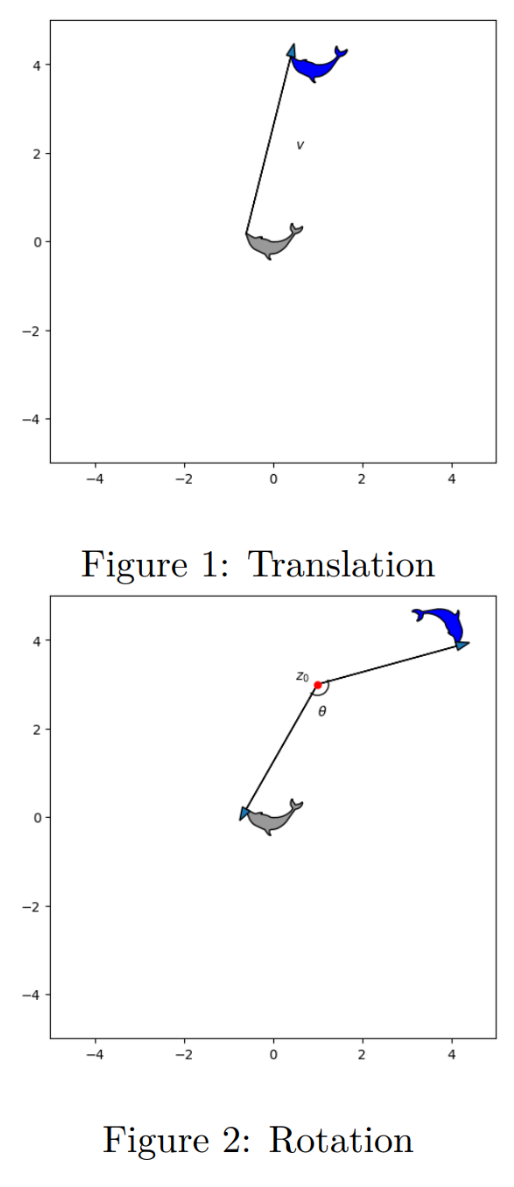
\includegraphics[width=0.5\linewidth]{Homework 2.png}
\end{figure}

Define the functions:
\begin{itemize}
    \item $f_v(z):$ translate $z$ by a vector $v\in\mathbb{R}^2$. 
    \item $g_{z_0,\theta}:$ rotate $z$ with respect to $z_0$ by angle $\theta$ counter-clockwise. 
\end{itemize}

\begin{definition}
    For two functions $f,g:\mathbb{R}^2\rightarrow\mathbb{R}^2$ \textit{commute}, if $$\forall z\in\mathbb{R}^2, f\circ g(z) = g\circ f(z).$$
\end{definition}
 Based on the above definition, determine if each of the following statements is true or false. Justify your answer. 
\question  $\forall v\in\mathbb{R}^2, \forall z_0\in\mathbb{R}^2, \forall\theta\in[0,2\pi), f_v$ and $g_{z_0,\theta}$ commute. 
\begin{proof}
    FALSE. Choose $v=(1,0)$, $z_0=(0,0)$, $\theta=\frac{\pi}2$. $f_v\circ g_{z_0,\theta}(0,0)=(1,0)$. $g\circ f(0,0)=(0,1)$.   
\end{proof}

\question $\exists v\in\mathbb{R}^2, \exists z_0\in\mathbb{R}^2, \exists\theta\in[0,2\pi), f_v$ and $g_{z_0,\theta}$ commute. 
\begin{proof}
    TRUE. Choose $v=(0,0), z_0=(0,0),\theta=0$, $f(0,0)=(0,0)=g(0,0)$. 
\end{proof}

\end{document}